\documentclass[runningheads]{llncs}

\usepackage{graphicx}
\usepackage{placeins}
\usepackage{hyperref,xcolor}
\renewcommand\UrlFont{\color{blue}\rmfamily}

\begin{document}

\title{Solving Combinatorial Puzzles with Parallel Evolutionary Algorithms \thanks{This work was supported by a private funding of Velbazhd Software LLC.}}
\titlerunning{Solving Puzzles with PEA}

\author{Todor Balabanov\orcidID{0000-0003-3139-069X} \and
Stoyan Ivanov \and
Rumen Ketipov}
\authorrunning{T. Balabanov et al.}

\institute{Institute of Information and Communication Technologies \\
Bulgarian Academy of Sciences \\
acad. Georgi Bonchev Str., Block 2, 1113 Sofia, Bulgaria \\
\email{todorb@iinf.bas.bg} \\
\url{http://iict.bas.bg/}}

\maketitle

\begin{abstract}
Rubik's cube is the most popular combinatorial puzzle. It is well known that solutions of the combinatorial problems are generally hard to find. If 90 degree clockwise rotations of the cube's sides are taken as operations it will give a minimal cube's grammar. By building formal grammar sentences with the usage of the six operations ([L]eft, [R]ight, [T]op, [D]own, [F]ront, [B]ack) all cube's permutations can be achieved. In an evolutionary algorithms (like genetic algorithms for example) set of formal grammar sentences can be represented as population individuals. Single cut point crossover can be efficiently applied when population individuals are strings. Changing randomly selected operation with another randomly selected operation can be used as efficient mutation operator. The most important part of such global optimization is the fitness function. For better individuals fitness value evaluation a combination between Euclidean and Hausdorff distances is proposed in this research. The experiments in this research are done as parallel program written in C++ and Open MPI.

\keywords{Distributed evolutionary algorithms \and Combinatorial puzzles \and Integer optimization.}
\end{abstract}

\section{Introduction}

A parallel implementation of a genetic algorithm based solver of the Rubik's cube was implemented by Balabanov in \cite{balabanov01} and it was presented in \cite{balabanov02}. Rubik's cube was invented and introduced by Erno Rubik in the 70s of the 20th century. After its creation the cube became the most popular combinatorial puzzle all over the world. In its original version it has 3x3x3 cubical segments. There are stickers in six different colors on each subcube square of the exposed sides. Each of the six planes (3x3x1) can be rotated in 90, 180, 270 or 360 degrees, relative to the other part of the puzzle. In the original initial state all sides of the cube are in single color. Scumbling of the puzzle is done by many random rotations of the (3x3x1) sides. The optimization task is to restore the cube in its original state. Such combinatorial optimization problem is quite difficult, because there are billions of combinations. The real number of combinations is $4.3252*10^{19}$ \cite{korf01} and all of them can be reached from any starting combination. The puzzle is successfully resolved when a sequence of moves is applied such that all subcubes are matched to each other by their color on each side of the cube. By estimation in \cite{korf01}, resolutions sequences variate from 50 to 100 moves when the cube is well scrambled. 

When there is an optimization problem with a sequence of commands it is a perfect candidate for evolutionary algorithms as optimizers. This research addresses the application of parallel genetic algorithms for Rubik's cube optimal or suboptimal solutions findings. The source code of the experiments is written in C++ with OpenMPI for parallel calculations and it can be found in a public source code repository \cite{balabanov01}. Modification of the evaluation function presented in \cite{balabanov02} is upgraded by addition of Hausdorff distance component.

The rest of this paper is organized as follows: Section 2 describes theoretical details. Section 3 presents the proposed modifications into a practical software example. Section 4 is devoted to some experiments and results. Finally, Section 5 concludes and presents some ideas for further research.

\section{Parallel Genetic Algorithms}

\section{Modified Rubik's Cube Solver}

The core of the optimization code is Rubik's cube representation into the computer memory. For the needs in this research the cube is presented as six (one for each side) two-dimensional (3x3) arrays. Values in these arrays are integer numbers which correspond to cube's colors. There are better ways for digital representation \cite{korf01}, but it is much more practical in this way from algorithmic aspect. 

Data structures are on first side of the modeling. On the second side are the algorithmic operations done over the data structures. The cube has six sides that is why the minimum number of operations over the cube is six. Six capital letters are used for 90 degrees clockwise rotations, as proposed in \cite{randall01,balabanov02}: \\ 
\\
T (Top) –90 degrees clockwise rotation of the top side; \\ 
L (Left) –90 degrees clockwise rotation of the left side; \\ 
B (Back) –90 degrees clockwise rotation of the back side; \\ 
R (Right) –90 degrees clockwise rotation of the right side; \\ 
F (Front) –90 degrees clockwise rotation of the front side; \\ 
D (Down) –90 degrees clockwise rotation of the down side. \\ 

This set of six operations is the minimal fully functional grammar for the Rubik's cube. Extended grammars are also possible, for example if counter-clockwise operators are included (+T, +L, +B, +R, +F, +D, –T, –L, –B, –R, –F, –D). Next level of extension is addition as number of turns (+1T, +2T, +3T, +1L, +2L, +3L, +1B, +2B, +3B, +1R, +2R, +3R, +1F, +2F, +3F, +1D,+2D, +3D, –1T, –2T, –3T, –1L, –2L, –3L, –1B, –2B, –3B, –1R, –2R, –3R, –1F, –2F, –3F, –1D, –2D, –3D) \cite{balabanov02}.

With this clear idea for a formal Rubik's cube grammar it is neutral genetic algorithm individuals to be represented as formal grammar sentences with variable length. Each of the letters can appear at any position many times repeated in the chromosome. As it was appointed in \cite{korf01} the average expected length of the chromosomes can be between 50 and 100.

\begin{figure}
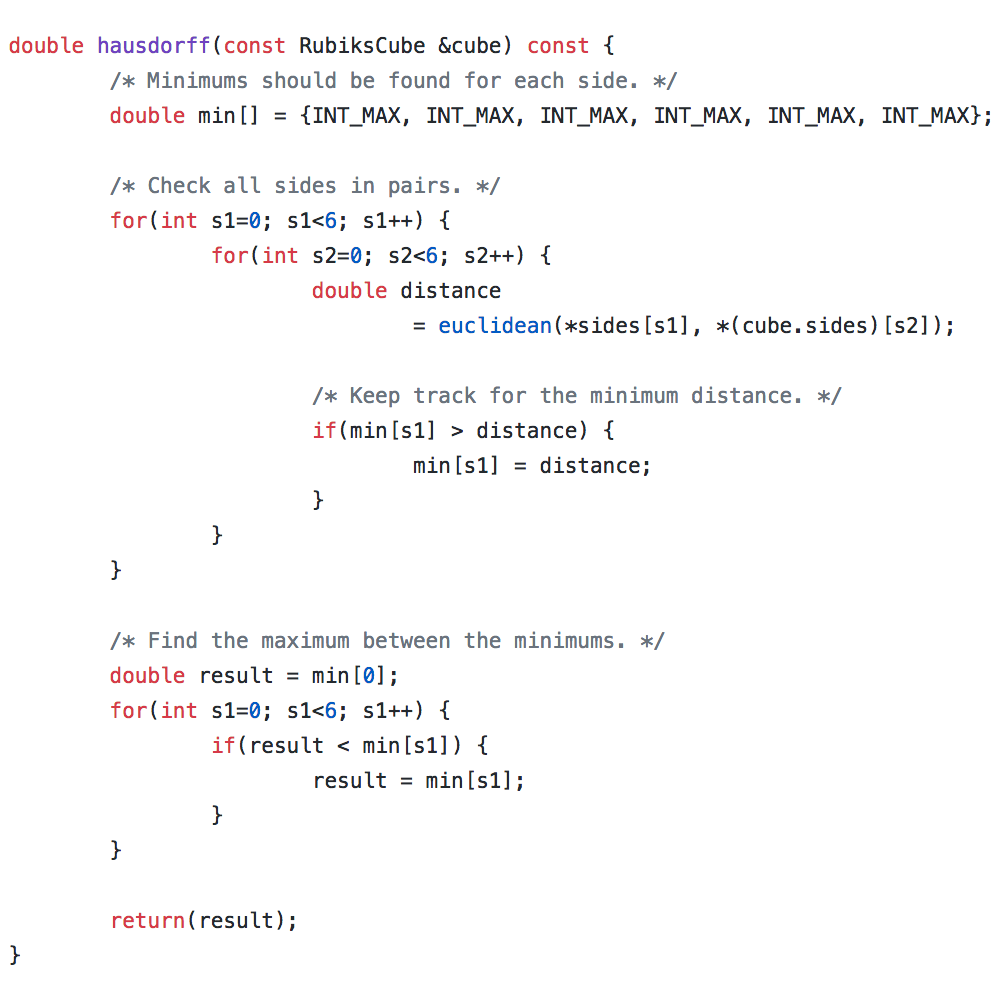
\includegraphics[width=\textwidth]{fig01.png}
\caption{Fitness value evaluation by combination between Euclidean and Hausdorff distance.} \label{fig01}
\end{figure}
\FloatBarrier

Single cut point is selected as crossover population, but other options \cite{poli01} are also applicable. As mutation operator random change of a single instruction is selected. Selection is done by randomly selected parents, but elitism rule is applied. For the evaluation of the newly created individuals instructions encoded in the individual are applied over the scrambled cube. After that the state of the cube is compared with the target state (cube in the solved state). The listing in Fig.\ref{fig01} shows the proposed in this paper modification of fitness evaluation function. For each pairs of cube's sides Euclidean distance is calculated. After that according Hausdorff distance rules the maximum of the minimums is found. Evaluated fitness value is positive, because the Euclidean distance is calculated with positive integers (cube's colors are mapped to integers) and the Hausdorff distance is calculation of a maximum of the minimums. The puzzle is as better solved as the fitness value is smaller. 

\section{Experiments and Results}

All experiments were done on a single processor desktop machine - Intel Core i5, 2.3 GHz, 2 Cores, 8GB RAM and Mac OS X 10.13.6, Apple LLVM version 9.1.0. For the parallel implementation Open MPI is used.

\section{Conclusions}

\cite{tashev01}

\cite{alexandrov01}

\cite{atanasova01}

\begin{thebibliography}{8}
\bibitem{balabanov01}
MPI Parallel Implementation of Genetic Algorithm Based Rubik’s Cube Solver, \url{http://github.com/TodorBalabanov/RubiksCubeGeneticAlgorithmsSolver}. Last accessed 12 Jan 2019
\bibitem{balabanov02}
Balabanov, T., Zankinski, I., Barova, M.: Strategy for Individuals Distribution by Incident Nodes Participation in Star Topology of Distributed Evolutionary Algorithms. Cybernetics and Information Technologies \textbf{16}(1), 80--88 (2016)
\bibitem{korf01}
Korf, R.: Finding Optimal Solutions to Rubik’s Cube Using Pattern Databases. In: AAAI-98 Proceedings, pp. 700--705. AAAI Press, Menlo Park, CA, USA (1998)
\bibitem{randall01}
Randall, K.: Cilk - Efficient Multithreaded Computing. Doctor of Philosophy Thesis in Computer Science and Engineering, Massachusetts Institute of Technology, USA (1998) 
\bibitem{poli01}
Poli, R., Kozak J.: Genetic Programming. In: Burke, EK., Kendall, G. (eds.) Search Methodologies, pp. 143--185. Springer US (2014)
\bibitem{tashev01}
Tashev, T., Hristov, H.: Modeling of synthesis of information processes with generalized nets. Cybernetics and Information Technologies, \textbf{3}(2), 92--104 (2003) 
\bibitem{alexandrov01}
Alexandrov, A.: AD HOC Kalman filter based fusion algorithm for real-time Wireless Sensor Data Integration. In: FQAS-2015 Proceedings, pp. 151--160. Springer, Heidelberg (2015)
\bibitem{atanasova01}
Atanasova T., Barova M.: Exploratory analysis of Time Series for hypothesize feature values. In: UniTech17 Proceedings,  \textbf{16}(2), 399--403 (2017)
\end{thebibliography}
\end{document}
